\documentclass[11pt]{amsart}
    \topmargin -.5 in
    \textheight 9.0in
    \textwidth 6.25 in
    \oddsidemargin 0 in
    \evensidemargin 0 in
   
\usepackage{amsmath}
\usepackage{enumerate}
\usepackage{tikz,tkz-graph}
%\usepackage{nth}

\newcommand{\ceil}[1]{\left\lceil#1\right\rceil}
\newcommand{\floor}[1]{\left\lfloor#1\right\rfloor}


\newenvironment{graph}[1][scale=1]{
\begin{tikzpicture}[#1]
\tikzstyle{vertex}=[circle, draw, fill, inner sep=0pt, minimum size=4pt]%
\tikzstyle{bigvtx}=[circle, draw, fill, inner sep=0pt, minimum size=6pt]%
\tikzstyle{every path}=[line width=0.5pt]%
}{\end{tikzpicture}}


\begin{document}
\title{Math 454\\ Homework 4 \qquad Due February 15}
\author{}
\date{}
\maketitle
\thispagestyle{empty}

\noindent Name:~\hrulefill~~\\

\begin{itemize}
\item Refer to the syllabus regarding allowed collaboration on this homework assignment.
\item Refer to other homework instructions and suggestions posted in Blackboard.
\item All answers must be fully justified.
\item Your homework should be neatly written on additional paper; you may attach this cover page if you would like to keep the questions attached to the answers.
\end{itemize}

\bigskip

Turn in four of the following problems to be graded.

\bigskip

\begin{enumerate}
\item (1.3.52)  Prove that $K_{\floor{n/2},\ceil{n/2}}$ is the only sharpness example for Mantel's Theorem.  That is, show that if $G$ is a triangle-free $n$-vertex simple graph and $e(G)=\floor{n^2/4}$, then $G\cong K_{\floor{n/2},\ceil{n/2}}$.  \textit{(Hint: follow the proof of Mantel's Theorem.  Knowing $e(G)$ allows you to conclude that some inequalities must be equalities.)}

\item 
\begin{enumerate}
\item (1.3.57)  Let $n\in\mathbb{N}$ and let $d$ be a list of $n$ nonnegative integers with even sum whose largest entry is less than $n$ and differs from the smallest entry by at most 1 (e.g., 443333 or 33333322).  Prove that $d$ is graphic.
\item Conclude that there is a $k$-regular $n$-vertex simple graph if and only if $k<n$ and $kn$ is even.  \textit{(Remark: it might not be so easy to prove this directly, especially by induction.  We  ``strengthened the induction hypothesis'' above to include more sequences, and the resulting induction was much easier.)}
\end{enumerate}

\item (1.3.63)  Let $d_1\geq d_2 \geq \dotsb \geq d_n \geq 0$.  Prove that there is a loopless graph (multiple edges allowed) with degree sequence $d_1, \dotsc, d_n$ if and only if $\sum d_i$ is even and $d_1\leq \frac12 \sum d_i$.

\medskip

\item (1.4.14) Let $D$ be an $n$-vertex digraph with no cycles.  Prove that the vertices of $D$ can be ordered as $v_1, \dotsc, v_n$ so that if $v_i\to v_j$, then $i<j$.

\item (1.4.23)   Prove that every graph $G$ has an orientation $D$ such that $\left|d^+_D(v)-d^-_D(v)\right|\leq1$. for every $v\in V(G)$.  \textit{(VagueHint\texttrademark: is $G$ Eulerian?)}

\item (1.4.26ish) Find a cyclic list of 16 bits so that the 16 strings of five consecutive bits are all the 5-bit strings with at least three 1's.  Explain your construction method.  \emph{(Hint: below is a drawing of $D_5$; use it.)}

\end{enumerate}

\begin{center}
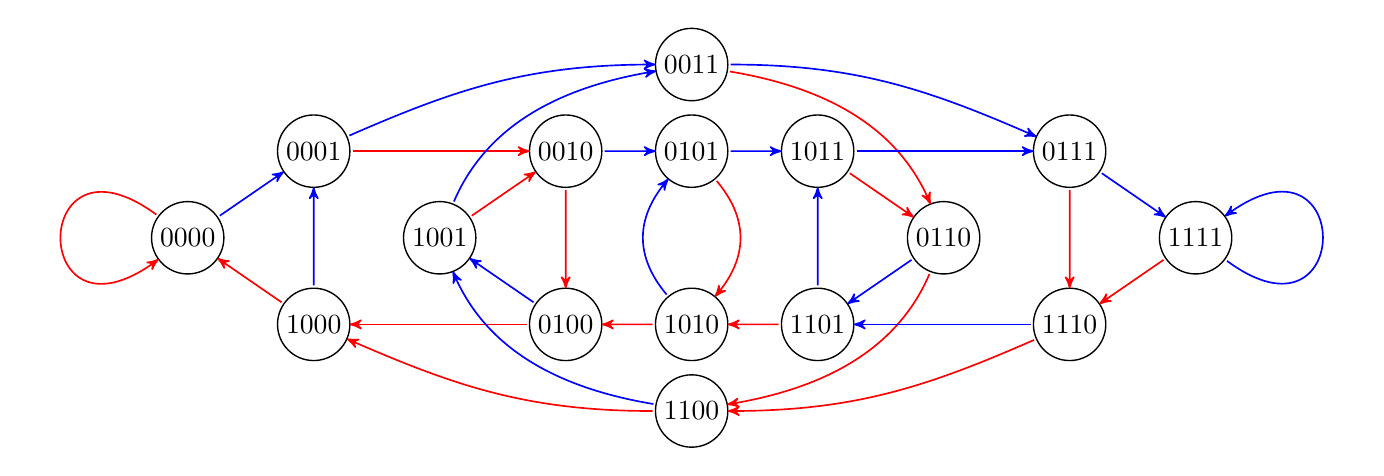
\begin{tikzpicture}[xscale=0.8,yscale=0.55]
\definecolor{cv0}{rgb}{0.0,0.0,0.0}
\definecolor{cfv0}{rgb}{1.0,1.0,1.0}
\definecolor{clv0}{rgb}{0.0,0.0,0.0}
\definecolor{cv1}{rgb}{0.0,0.0,0.0}
\definecolor{cfv1}{rgb}{1.0,1.0,1.0}
\definecolor{clv1}{rgb}{0.0,0.0,0.0}
\definecolor{cv2}{rgb}{0.0,0.0,0.0}
\definecolor{cfv2}{rgb}{1.0,1.0,1.0}
\definecolor{clv2}{rgb}{0.0,0.0,0.0}
\definecolor{cv3}{rgb}{0.0,0.0,0.0}
\definecolor{cfv3}{rgb}{1.0,1.0,1.0}
\definecolor{clv3}{rgb}{0.0,0.0,0.0}
\definecolor{cv4}{rgb}{0.0,0.0,0.0}
\definecolor{cfv4}{rgb}{1.0,1.0,1.0}
\definecolor{clv4}{rgb}{0.0,0.0,0.0}
\definecolor{cv5}{rgb}{0.0,0.0,0.0}
\definecolor{cfv5}{rgb}{1.0,1.0,1.0}
\definecolor{clv5}{rgb}{0.0,0.0,0.0}
\definecolor{cv6}{rgb}{0.0,0.0,0.0}
\definecolor{cfv6}{rgb}{1.0,1.0,1.0}
\definecolor{clv6}{rgb}{0.0,0.0,0.0}
\definecolor{cv7}{rgb}{0.0,0.0,0.0}
\definecolor{cfv7}{rgb}{1.0,1.0,1.0}
\definecolor{clv7}{rgb}{0.0,0.0,0.0}
\definecolor{cv8}{rgb}{0.0,0.0,0.0}
\definecolor{cfv8}{rgb}{1.0,1.0,1.0}
\definecolor{clv8}{rgb}{0.0,0.0,0.0}
\definecolor{cv9}{rgb}{0.0,0.0,0.0}
\definecolor{cfv9}{rgb}{1.0,1.0,1.0}
\definecolor{clv9}{rgb}{0.0,0.0,0.0}
\definecolor{cv10}{rgb}{0.0,0.0,0.0}
\definecolor{cfv10}{rgb}{1.0,1.0,1.0}
\definecolor{clv10}{rgb}{0.0,0.0,0.0}
\definecolor{cv11}{rgb}{0.0,0.0,0.0}
\definecolor{cfv11}{rgb}{1.0,1.0,1.0}
\definecolor{clv11}{rgb}{0.0,0.0,0.0}
\definecolor{cv12}{rgb}{0.0,0.0,0.0}
\definecolor{cfv12}{rgb}{1.0,1.0,1.0}
\definecolor{clv12}{rgb}{0.0,0.0,0.0}
\definecolor{cv13}{rgb}{0.0,0.0,0.0}
\definecolor{cfv13}{rgb}{1.0,1.0,1.0}
\definecolor{clv13}{rgb}{0.0,0.0,0.0}
\definecolor{cv14}{rgb}{0.0,0.0,0.0}
\definecolor{cfv14}{rgb}{1.0,1.0,1.0}
\definecolor{clv14}{rgb}{0.0,0.0,0.0}
\definecolor{cv15}{rgb}{0.0,0.0,0.0}
\definecolor{cfv15}{rgb}{1.0,1.0,1.0}
\definecolor{clv15}{rgb}{0.0,0.0,0.0}
\definecolor{cv0v0}{rgb}{1.0,0.0,0.0}
\definecolor{cv0v1}{rgb}{0.0,0.0,1.0}
\definecolor{cv1v2}{rgb}{1.0,0.0,0.0}
\definecolor{cv1v3}{rgb}{0.0,0.0,1.0}
\definecolor{cv2v4}{rgb}{1.0,0.0,0.0}
\definecolor{cv2v5}{rgb}{0.0,0.0,1.0}
\definecolor{cv3v6}{rgb}{1.0,0.0,0.0}
\definecolor{cv3v7}{rgb}{0.0,0.0,1.0}
\definecolor{cv4v8}{rgb}{1.0,0.0,0.0}
\definecolor{cv4v9}{rgb}{0.0,0.0,1.0}
\definecolor{cv5v10}{rgb}{1.0,0.0,0.0}
\definecolor{cv5v11}{rgb}{0.0,0.0,1.0}
\definecolor{cv6v12}{rgb}{1.0,0.0,0.0}
\definecolor{cv6v13}{rgb}{0.0,0.0,1.0}
\definecolor{cv7v14}{rgb}{1.0,0.0,0.0}
\definecolor{cv7v15}{rgb}{0.0,0.0,1.0}
\definecolor{cv8v0}{rgb}{1.0,0.0,0.0}
\definecolor{cv8v1}{rgb}{0.0,0.0,1.0}
\definecolor{cv9v2}{rgb}{1.0,0.0,0.0}
\definecolor{cv9v3}{rgb}{0.0,0.0,1.0}
\definecolor{cv10v4}{rgb}{1.0,0.0,0.0}
\definecolor{cv10v5}{rgb}{0.0,0.0,1.0}
\definecolor{cv11v6}{rgb}{1.0,0.0,0.0}
\definecolor{cv11v7}{rgb}{0.0,0.0,1.0}
\definecolor{cv12v8}{rgb}{1.0,0.0,0.0}
\definecolor{cv12v9}{rgb}{0.0,0.0,1.0}
\definecolor{cv13v10}{rgb}{1.0,0.0,0.0}
\definecolor{cv13v11}{rgb}{0.0,0.0,1.0}
\definecolor{cv14v12}{rgb}{1.0,0.0,0.0}
\definecolor{cv14v13}{rgb}{0.0,0.0,1.0}
\definecolor{cv15v14}{rgb}{1.0,0.0,0.0}
\definecolor{cv15v15}{rgb}{0.0,0.0,1.0}
%
\Vertex[style={minimum size=1.0cm,draw=cv0,fill=cfv0,text=clv0,shape=circle},LabelOut=false,L=\hbox{$0000$},x=0,y=0]{v0}
\Vertex[style={minimum size=1.0cm,draw=cv1,fill=cfv1,text=clv1,shape=circle},LabelOut=false,L=\hbox{$0001$},x=2,y=2]{v1}
\Vertex[style={minimum size=1.0cm,draw=cv2,fill=cfv2,text=clv2,shape=circle},LabelOut=false,L=\hbox{$0010$},x=6,y=2]{v2}
\Vertex[style={minimum size=1.0cm,draw=cv3,fill=cfv3,text=clv3,shape=circle},LabelOut=false,L=\hbox{$0011$},x=8,y=4]{v3}
\Vertex[style={minimum size=1.0cm,draw=cv4,fill=cfv4,text=clv4,shape=circle},LabelOut=false,L=\hbox{$0100$},x=6,y=-2]{v4}
\Vertex[style={minimum size=1.0cm,draw=cv5,fill=cfv5,text=clv5,shape=circle},LabelOut=false,L=\hbox{$0101$},x=8,y=2]{v5}
\Vertex[style={minimum size=1.0cm,draw=cv6,fill=cfv6,text=clv6,shape=circle},LabelOut=false,L=\hbox{$0110$},x=12,y=0]{v6}
\Vertex[style={minimum size=1.0cm,draw=cv7,fill=cfv7,text=clv7,shape=circle},LabelOut=false,L=\hbox{$0111$},x=14,y=2]{v7}
\Vertex[style={minimum size=1.0cm,draw=cv8,fill=cfv8,text=clv8,shape=circle},LabelOut=false,L=\hbox{$1000$},x=2,y=-2]{v8}
\Vertex[style={minimum size=1.0cm,draw=cv9,fill=cfv9,text=clv9,shape=circle},LabelOut=false,L=\hbox{$1001$},x=4,y=0]{v9}
\Vertex[style={minimum size=1.0cm,draw=cv10,fill=cfv10,text=clv10,shape=circle},LabelOut=false,L=\hbox{$1010$},x=8,y=-2]{v10}
\Vertex[style={minimum size=1.0cm,draw=cv11,fill=cfv11,text=clv11,shape=circle},LabelOut=false,L=\hbox{$1011$},x=10,y=2]{v11}
\Vertex[style={minimum size=1.0cm,draw=cv12,fill=cfv12,text=clv12,shape=circle},LabelOut=false,L=\hbox{$1100$},x=8,y=-4]{v12}
\Vertex[style={minimum size=1.0cm,draw=cv13,fill=cfv13,text=clv13,shape=circle},LabelOut=false,L=\hbox{$1101$},x=10,y=-2]{v13}
\Vertex[style={minimum size=1.0cm,draw=cv14,fill=cfv14,text=clv14,shape=circle},LabelOut=false,L=\hbox{$1110$},x=14,y=-2]{v14}
\Vertex[style={minimum size=1.0cm,draw=cv15,fill=cfv15,text=clv15,shape=circle},LabelOut=false,L=\hbox{$1111$},x=16,y=0]{v15}
%
\Loop[dist=3.0cm,dir=WE,style={post,color=cv0v0,},](v0)
\Edge[lw=0.1cm,style={post,color=cv0v1,},](v0)(v1)
\Edge[lw=0.1cm,style={post,color=cv1v2,},](v1)(v2)
\Edge[lw=0.1cm,style={post,out=30,in=180,color=cv1v3,},](v1)(v3)
\Edge[lw=0.1cm,style={post,color=cv2v4,},](v2)(v4)
\Edge[lw=0.1cm,style={post,color=cv2v5,},](v2)(v5)
\Edge[lw=0.1cm,style={post,bend left,color=cv3v6,},](v3)(v6)
\Edge[lw=0.1cm,style={post,out=0,in=150,color=cv3v7,},](v3)(v7)
\Edge[lw=0.1cm,style={post,color=cv4v8,},](v4)(v8)
\Edge[lw=0.1cm,style={post,color=cv4v9,},](v4)(v9)
\Edge[lw=0.1cm,style={post,bend left,color=cv5v10,},](v5)(v10)
\Edge[lw=0.1cm,style={post,color=cv5v11,},](v5)(v11)
\Edge[lw=0.1cm,style={post,bend left,color=cv6v12,},](v6)(v12)
\Edge[lw=0.1cm,style={post,color=cv6v13,},](v6)(v13)
\Edge[lw=0.1cm,style={post,color=cv7v14,},](v7)(v14)
\Edge[lw=0.1cm,style={post,color=cv7v15,},](v7)(v15)
\Edge[lw=0.1cm,style={post,color=cv8v0,},](v8)(v0)
\Edge[lw=0.1cm,style={post,color=cv8v1,},](v8)(v1)
\Edge[lw=0.1cm,style={post,color=cv9v2,},](v9)(v2)
\Edge[lw=0.1cm,style={post,bend left,color=cv9v3,},](v9)(v3)
\Edge[lw=0.1cm,style={post,color=cv10v4,},](v10)(v4)
\Edge[lw=0.1cm,style={post,bend left,color=cv10v5,},](v10)(v5)
\Edge[lw=0.1cm,style={post,color=cv11v6,},](v11)(v6)
\Edge[lw=0.1cm,style={post,color=cv11v7,},](v11)(v7)
\Edge[lw=0.1cm,style={post,out=180,in=-30,color=cv12v8,},](v12)(v8)
\Edge[lw=0.1cm,style={post,bend left,color=cv12v9,},](v12)(v9)
\Edge[lw=0.1cm,style={post,color=cv13v10,},](v13)(v10)
\Edge[lw=0.1cm,style={post,color=cv13v11,},](v13)(v11)
\Edge[lw=0.1cm,style={post,out=210,in=0,color=cv14v12,},](v14)(v12)
\Edge[lw=0.1cm,style={post,color=cv14v13,},](v14)(v13)
\Edge[lw=0.1cm,style={post,color=cv15v14,},](v15)(v14)
\Loop[dist=3.0cm,dir=EA,style={post,color=cv15v15,},](v15)
%
\end{tikzpicture}
\end{center}



%\vfill
%\begin{quotation}
%\footnotesize
%\end{quotation}

\end{document}

